\documentclass[8pt,aspectratio=169]{beamer}
\usetheme{Madrid}
\usepackage{graphicx}
\usepackage{booktabs}
\usepackage{adjustbox}
\usepackage{multicol}
\usepackage{amsmath}
\usepackage{amssymb}
\usepackage{tikz}
\usepackage{hyperref}
\usepackage{algorithm}
\usepackage{algorithmic}
\usepackage{colortbl}
\usepackage{pgfplots}
\pgfplotsset{compat=1.18}

% TikZ libraries for comics, diagrams, stakeholder maps
\usetikzlibrary{arrows.meta,positioning,shapes.callouts,shapes.geometric,decorations.pathreplacing}

% Color definitions
\definecolor{mlblue}{RGB}{0,102,204}
\definecolor{mlpurple}{RGB}{51,51,178}
\definecolor{mllavender}{RGB}{173,173,224}
\definecolor{mllavender2}{RGB}{193,193,232}
\definecolor{mllavender3}{RGB}{204,204,235}
\definecolor{mllavender4}{RGB}{214,214,239}
\definecolor{mlorange}{RGB}{255, 127, 14}
\definecolor{mlgreen}{RGB}{44, 160, 44}
\definecolor{mlred}{RGB}{214, 39, 40}
\definecolor{mlgray}{RGB}{127, 127, 127}
\definecolor{lightgray}{RGB}{240, 240, 240}
\definecolor{midgray}{RGB}{180, 180, 180}

% NEW COLORS for mini-lecture
\definecolor{dfteal}{RGB}{0,128,128}
\definecolor{dfred}{RGB}{180,30,30}

% Backward compatibility
\colorlet{MLPurple}{mlpurple}
\colorlet{MLBlue}{mlblue}
\colorlet{MLOrange}{mlorange}
\colorlet{MLGreen}{mlgreen}
\colorlet{MLRed}{mlred}
\colorlet{MLLavender}{mllavender}
\colorlet{MLGray}{mlgray}

% Theme colors (exact Madrid settings)
\setbeamercolor{palette primary}{bg=mllavender3,fg=mlpurple}
\setbeamercolor{palette secondary}{bg=mllavender2,fg=mlpurple}
\setbeamercolor{palette tertiary}{bg=mllavender,fg=white}
\setbeamercolor{palette quaternary}{bg=mlpurple,fg=white}
\setbeamercolor{structure}{fg=mlpurple}
\setbeamercolor{section in toc}{fg=mlpurple}
\setbeamercolor{subsection in toc}{fg=mlblue}
\setbeamercolor{title}{fg=mlpurple}
\setbeamercolor{frametitle}{fg=mlpurple,bg=mllavender3}
\setbeamercolor{block title}{bg=mllavender2,fg=mlpurple}
\setbeamercolor{block body}{bg=mllavender4,fg=black}
\setbeamertemplate{navigation symbols}{}
\setbeamertemplate{itemize items}[circle]
\setbeamertemplate{enumerate items}[default]
\setbeamersize{text margin left=5mm,text margin right=5mm}

% Footer
\setbeamertemplate{footline}{
  \leavevmode%
  \hbox{%
    \begin{beamercolorbox}[wd=.333333\paperwidth,ht=2.25ex,dp=1ex,center]{author in head/foot}%
      \usebeamerfont{author in head/foot}Methods and Algorithms
    \end{beamercolorbox}%
    \begin{beamercolorbox}[wd=.333333\paperwidth,ht=2.25ex,dp=1ex,center]{title in head/foot}%
      \usebeamerfont{title in head/foot}MSc Data Science
    \end{beamercolorbox}%
    \begin{beamercolorbox}[wd=.333333\paperwidth,ht=2.25ex,dp=1ex,right]{date in head/foot}%
      \usebeamerfont{date in head/foot}\insertframenumber{} / \inserttotalframenumber\hspace*{2ex}
    \end{beamercolorbox}}%
  \vskip0pt%
}

\newcommand{\bottomnote}[1]{%
\vfill
\vspace{-2mm}
\textcolor{mllavender2}{\rule{\textwidth}{0.4pt}}
\vspace{1mm}
\footnotesize
\textbf{#1}
}

\newenvironment{compactlist}{%
  \begin{itemize}%
    \setlength{\itemsep}{2pt}%
    \setlength{\parskip}{0pt}%
    \setlength{\parsep}{0pt}%
}{%
  \end{itemize}%
}

\newcommand{\highlight}[1]{\textcolor{mlorange}{\textbf{#1}}}
\newcommand{\mathbold}[1]{\boldsymbol{#1}}

\title[L04: Random Forests Full Lecture]{L04: Random Forests}
\subtitle{Full Lecture: Ensemble Learning, Variance Reduction, and Fraud Detection}
\author{Methods and Algorithms}
\institute{MSc Data Science}
\date{}

\begin{document}

%% === SECTION 0: OPENING ===

% Frame 1: Title
\begin{frame}
\titlepage
\end{frame}

% Frame 2: The Ensemble Approach
\begin{frame}{The Ensemble Approach}
\begin{columns}[T]
\begin{column}{0.55\textwidth}
\small
The cartoon captures the absurdity -- and power -- of combining models.

\vspace{0.5em}
\begin{compactlist}
\item One model is fragile; many models are robust
\item Ensembles exploit the \highlight{wisdom of crowds}: independent errors cancel
\item Random Forests, boosting, and stacking all follow this principle
\item The key insight: \highlight{diversity} among models matters more than individual accuracy
\end{compactlist}
\end{column}
\begin{column}{0.42\textwidth}
\includegraphics[height=0.55\textheight]{images/1885_ensemble_model.png}
\end{column}
\end{columns}
\bottomnote{XKCD \#1885 by Randall Munroe (CC BY-NC 2.5)}
\end{frame}

% Frame 3: Learning Objectives
\begin{frame}{Learning Objectives}
\begin{columns}[T]
\begin{column}{0.55\textwidth}
\small
By the end of this lecture, you will be able to:
\begin{enumerate}
\setlength{\itemsep}{4pt}
\item \textbf{Derive} the variance reduction formula for ensemble averaging (Analyze)
\item \textbf{Evaluate} RF vs.\ boosting through the bias-variance lens (Evaluate)
\item \textbf{Analyze} feature importance: MDI, permutation, SHAP (Analyze)
\item \textbf{Apply} ensembles to fraud detection with class imbalance (Apply)
\item \textbf{Compare} RF, AdaBoost, gradient boosting, XGBoost (Evaluate)
\end{enumerate}
\end{column}
\begin{column}{0.42\textwidth}
\small
\begin{block}{Bloom's Taxonomy Levels}
\begin{compactlist}
\item \textcolor{mlblue}{Analyze} -- break down, derive, compare components
\item \textcolor{mlgreen}{Evaluate} -- judge tradeoffs, assess suitability
\item \textcolor{mlorange}{Apply} -- use methods on real data problems
\end{compactlist}
\end{block}
\end{column}
\end{columns}
\bottomnote{L04 covers ensemble methods from bagging to boosting with finance applications.}
\end{frame}

%% === SECTION 1: DECISION TREES ===

% Frame 4: Why Would a Single Tree Overfit Every Dataset It Touches?
\begin{frame}{Why Would a Single Tree Overfit Every Dataset It Touches?}
\begin{columns}[T]
\begin{column}{0.55\textwidth}
\small
\begin{compactlist}
\item A fully grown tree has \highlight{low bias} (fits training data perfectly)
\item But \highlight{high variance}: small data changes produce entirely different trees
\item Bias-variance decomposition: $\text{MSE} = \text{Bias}^2 + \text{Variance} + \text{Noise}$
\item Trees are \highlight{unstable learners} -- ideal building blocks for ensembles
\end{compactlist}
\end{column}
\begin{column}{0.42\textwidth}
\scriptsize
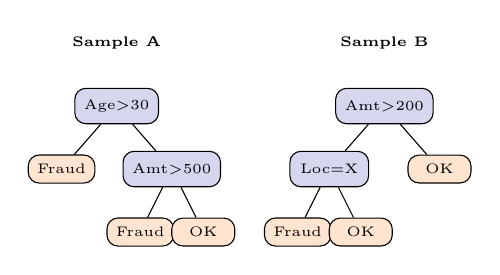
\begin{tikzpicture}[
  every node/.style={font=\tiny},
  treenode/.style={draw,rounded corners,fill=mllavender4,minimum width=1cm,minimum height=0.45cm,align=center},
  leafnode/.style={draw,rounded corners,fill=mlorange!20,minimum width=0.8cm,minimum height=0.35cm,align=center},
  level 1/.style={sibling distance=1.4cm,level distance=0.8cm},
  level 2/.style={sibling distance=0.8cm,level distance=0.8cm},
  arr/.style={->,>=stealth,thick}
]
% Sample A
\node[font=\tiny\bfseries] at (0,1) {Sample A};
\node[treenode] (a1) at (0,0.2) {Age$>$30}
  child {node[leafnode] {Fraud} }
  child {node[treenode] {Amt$>$500}
    child {node[leafnode] {Fraud}}
    child {node[leafnode] {OK}}
  };
% Sample B
\node[font=\tiny\bfseries] at (3.4,1) {Sample B};
\node[treenode] (b1) at (3.4,0.2) {Amt$>$200}
  child {node[treenode] {Loc=X}
    child {node[leafnode] {Fraud}}
    child {node[leafnode] {OK}}
  }
  child {node[leafnode] {OK} };
\end{tikzpicture}

\vspace{0.3em}
\scriptsize Different training samples $\Rightarrow$ completely different tree structures.
\end{column}
\end{columns}

\begin{block}{Insight}
\scriptsize High variance is a \emph{feature}, not a bug -- it means trees are sensitive enough to be improved by averaging.
\end{block}
\bottomnote{Unstable learners benefit most from ensemble methods (Breiman, 1996).}
\end{frame}

% Frame 5: How Does a Tree Choose the Best Split? (Gini Impurity)
\begin{frame}{How Does a Tree Choose the Best Split? (Gini Impurity)}
\begin{columns}[T]
\begin{column}{0.55\textwidth}
\small
\textbf{Gini Impurity} measures how often a random sample would be misclassified:
\[
G = 1 - \sum_{k=1}^{K} p_k^2
\]

\vspace{0.3em}
\footnotesize
\textbf{Binary case:} $G = 2p(1-p)$

\vspace{0.3em}
\textbf{Worked example (fraud data):}
\begin{compactlist}
\item Node: 800 legit, 200 fraud $\Rightarrow p_{\text{fraud}}=0.2$
\item $G = 1 - (0.8^2 + 0.2^2) = 1 - 0.68 = 0.32$
\item Best split minimizes weighted Gini of children
\end{compactlist}
\end{column}
\begin{column}{0.42\textwidth}
\footnotesize
\textbf{Split evaluation:}
\begin{compactlist}
\item Left child: 50 fraud / 100 total $\Rightarrow G_L = 0.50$
\item Right child: 150 fraud / 900 total $\Rightarrow G_R = 0.28$
\item Weighted: $\frac{100}{1000}(0.50) + \frac{900}{1000}(0.28) = 0.30$
\item Gain: $0.32 - 0.30 = 0.02$
\end{compactlist}

\vspace{0.3em}
\textbf{Properties:}
\begin{compactlist}
\item $G = 0$: pure node (one class only)
\item $G = 0.5$: maximum impurity (binary)
\item Computationally cheaper than entropy
\end{compactlist}
\end{column}
\end{columns}

\begin{block}{Insight}
\scriptsize Gini impurity is a \emph{concave} function of class proportions -- every split on a mixed node reduces impurity.
\end{block}
\bottomnote{CART uses Gini by default; scikit-learn's DecisionTreeClassifier(criterion='gini').}
\end{frame}

% Frame 6: What Does Entropy Add Beyond Gini?
\begin{frame}{What Does Entropy Add Beyond Gini?}
\begin{columns}[T]
\begin{column}{0.55\textwidth}
\small
\textbf{Shannon Entropy:}
\[
H = -\sum_{k=1}^{K} p_k \log_2 p_k
\]

\vspace{0.3em}
\footnotesize
\textbf{Information Gain:}
\[
\text{IG} = H(\text{parent}) - \sum_{j} \frac{n_j}{n}\,H(\text{child}_j)
\]

\vspace{0.3em}
\begin{compactlist}
\item Entropy is zero for pure nodes, maximal at uniform distribution
\item IG selects the feature that reduces uncertainty the most
\item C4.5 and ID3 algorithms use entropy; CART uses Gini
\item \highlight{Regression trees:} use MSE reduction (variance reduction) as the splitting criterion instead of Gini/Entropy
\end{compactlist}
\end{column}
\begin{column}{0.42\textwidth}
\footnotesize
\textbf{Gini vs.\ Entropy Comparison:}

\vspace{0.3em}
\renewcommand{\arraystretch}{1.2}
\begin{tabular}{@{}lcc@{}}
\toprule
\textbf{Property} & \textbf{Gini} & \textbf{Entropy} \\
\midrule
Range (binary) & $[0, 0.5]$ & $[0, 1]$ \\
Computation & Faster & $\log$ needed \\
Sensitivity & Majority class & Rare classes \\
Algorithm & CART & C4.5, ID3 \\
\bottomrule
\end{tabular}

\vspace{0.5em}
In practice, Gini and entropy produce \highlight{nearly identical} trees.
\end{column}
\end{columns}

\begin{block}{Insight}
\scriptsize Entropy penalizes impure nodes slightly more than Gini -- in fraud detection, this can surface rare-class splits earlier.
\end{block}
\bottomnote{For binary classification, $H \approx 2G$ near $p=0.5$; the choice rarely changes the final tree.}
\end{frame}

% Frame 7: What Does a Trained Decision Tree Actually Look Like?
\begin{frame}{What Does a Trained Decision Tree Actually Look Like?}
\begin{columns}[T]
\begin{column}{0.55\textwidth}
\small
\textbf{What you see:} A tree trained on financial features, splitting recursively on the most informative thresholds.

\vspace{0.3em}
\footnotesize
\textbf{Key pattern:} Each internal node tests one feature; each leaf assigns a class or value. Deeper trees fit noise.

\vspace{0.3em}
\textbf{Takeaway:} A single tree is interpretable but brittle -- small data shifts change the entire structure.
\end{column}
\begin{column}{0.42\textwidth}
\includegraphics[width=\textwidth]{01_decision_tree/chart.pdf}
\end{column}
\end{columns}

\begin{block}{Insight}
\scriptsize Interpretability is the single tree's greatest strength -- and its fragility is the motivation for ensembles.
\end{block}
\bottomnote{Pruning (max\_depth, min\_samples\_leaf) trades bias for variance reduction.}
\end{frame}

%% === SECTION 2: BAGGING ===

% Frame 8: Why Does Averaging Multiple Models Reduce Variance?
\begin{frame}{Why Does Averaging Multiple Models Reduce Variance?}
\begin{columns}[T]
\begin{column}{0.55\textwidth}
\small
\textbf{Key derivation.} For $B$ models with variance $\sigma^2$ and pairwise correlation $\rho$:
\[
\text{Var}\!\left(\frac{1}{B}\sum_{b=1}^{B} X_b\right) = \rho\sigma^2 + \frac{1-\rho}{B}\,\sigma^2
\]

\vspace{0.3em}
\footnotesize
\textbf{Two extreme cases:}
\begin{compactlist}
\item $\rho = 1$ (identical models): $\text{Var} = \sigma^2$ -- no improvement
\item $\rho = 0$ (independent models): $\text{Var} = \sigma^2 / B$ -- perfect scaling
\end{compactlist}

\vspace{0.3em}
The \highlight{goal of bagging}: reduce $\rho$ by training on different bootstrap samples while keeping $\sigma^2$ large (deep trees).
\end{column}
\begin{column}{0.42\textwidth}
\footnotesize
\textbf{Derivation sketch:}
\begin{compactlist}
\item $\text{Var}(\bar{X}) = \frac{1}{B^2}\sum_{i,j}\text{Cov}(X_i,X_j)$
\item Diagonal terms: $B \cdot \sigma^2$
\item Off-diagonal: $B(B-1)\rho\sigma^2$
\item Combine: $\frac{1}{B^2}[B\sigma^2 + B(B-1)\rho\sigma^2]$
\item Simplify to the variance formula above
\end{compactlist}

\vspace{0.5em}
\textbf{Practical implication:}\\
With $B=500$ and $\rho=0.05$:\\
$\text{Var} \approx 0.05\sigma^2 + \frac{0.95}{500}\sigma^2 \approx 0.052\sigma^2$
\end{column}
\end{columns}

\begin{block}{Insight}
\scriptsize The first term $\rho\sigma^2$ cannot be reduced by adding more trees -- only \emph{decorrelation} can shrink it.
\end{block}
\bottomnote{This is why Random Forests add feature randomization on top of bagging.}
\end{frame}

% Frame 9: How Does Bootstrap Sampling Create Diversity?
\begin{frame}{How Does Bootstrap Sampling Create Diversity?}
\begin{columns}[T]
\begin{column}{0.55\textwidth}
\small
\textbf{What you see:} Bootstrap resampling draws $n$ samples with replacement from $n$ observations.

\vspace{0.3em}
\footnotesize
\textbf{Key pattern:} Each bootstrap sample contains $\sim$63.2\% unique observations; the remaining $\sim$36.8\% are left out (OOB).

\vspace{0.3em}
\textbf{Takeaway:} Bootstrap creates model diversity through data perturbation -- each tree sees a different ``view'' of the training set.

\vspace{0.3em}
\begin{compactlist}
\item $P(\text{not selected}) = (1 - 1/n)^n \to 1/e \approx 0.368$
\item Duplicates force trees to emphasize different patterns
\item OOB samples become free validation data
\end{compactlist}
\end{column}
\begin{column}{0.42\textwidth}
\includegraphics[width=\textwidth]{03_bootstrap/chart.pdf}
\end{column}
\end{columns}

\begin{block}{Insight}
\scriptsize Bootstrap is a ``poor man's'' way to approximate drawing from the true data-generating distribution.
\end{block}
\bottomnote{Efron (1979) introduced bootstrap; Breiman (1996) applied it to tree ensembles.}
\end{frame}

% Frame 10: What Happens to the 36.8% of Samples Left Out?
\begin{frame}{What Happens to the 36.8\% of Samples Left Out?}
\begin{columns}[T]
\begin{column}{0.55\textwidth}
\small
\textbf{What you see:} OOB error converges as the number of trees grows, providing a built-in cross-validation estimate.

\vspace{0.3em}
\footnotesize
\textbf{Key pattern:} Each observation is OOB for $\sim$36.8\% of trees. Aggregate their predictions to get an unbiased error estimate.

\vspace{0.3em}
\textbf{Takeaway:} OOB error eliminates the need for a separate validation set -- especially valuable when data is scarce.

\vspace{0.3em}
\begin{compactlist}
\item OOB error $\approx$ leave-one-out CV error
\item No data ``wasted'' on validation
\item Monitored automatically in scikit-learn with \texttt{oob\_score=True}
\end{compactlist}
\end{column}
\begin{column}{0.42\textwidth}
\includegraphics[width=\textwidth]{04_oob_error/chart.pdf}
\end{column}
\end{columns}

\begin{block}{Insight}
\scriptsize OOB error is slightly pessimistic (each tree trained on $\sim$63\% of data), making it a conservative estimate.
\end{block}
\bottomnote{OOB error is one of Random Forests' most elegant properties -- free, unbiased validation.}
\end{frame}

%% === SECTION 3: RANDOM FORESTS ===

% Frame 11: What Is the One Trick That Makes Random Forests Better Than Bagging?
\begin{frame}{What Is the One Trick That Makes Random Forests Better Than Bagging?}
\begin{columns}[T]
\begin{column}{0.55\textwidth}
\small
\textbf{Feature randomization.} At each split, consider only a random subset of features:
\begin{compactlist}
\item Classification: $m = \lfloor\sqrt{p}\rfloor$
\item Regression: $m = \lfloor p/3 \rfloor$
\item This forces trees to use \highlight{different features}, reducing correlation $\rho$
\end{compactlist}

\vspace{0.3em}
\footnotesize
\textbf{Why it works:}
\begin{compactlist}
\item Without randomization, every tree splits on the same dominant feature first
\item Correlated trees $\Rightarrow$ correlated errors $\Rightarrow$ averaging helps less
\item Feature subsampling \highlight{decorrelates} the trees
\end{compactlist}
\end{column}
\begin{column}{0.42\textwidth}
\scriptsize
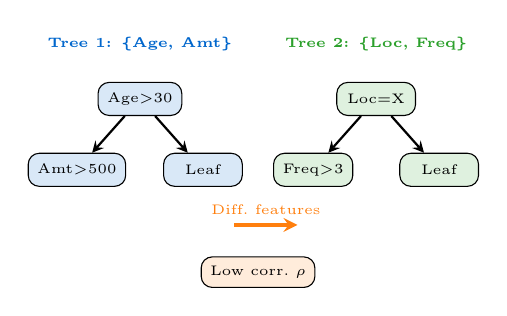
\begin{tikzpicture}[
  every node/.style={font=\tiny},
  treenode/.style={draw,rounded corners,fill=mllavender4,minimum width=1cm,minimum height=0.42cm,align=center},
  arr/.style={->,>=stealth,thick}
]
% Tree 1
\node[font=\tiny\bfseries,mlblue] at (0,2.3) {Tree 1: \{Age, Amt\}};
\node[treenode,fill=mlblue!15] (t1) at (0,1.6) {Age$>$30};
\node[treenode,fill=mlblue!15] (t1l) at (-0.8,0.7) {Amt$>$500};
\node[treenode,fill=mlblue!15] (t1r) at (0.8,0.7) {Leaf};
\draw[arr] (t1) -- (t1l);
\draw[arr] (t1) -- (t1r);

% Tree 2
\node[font=\tiny\bfseries,mlgreen] at (3.0,2.3) {Tree 2: \{Loc, Freq\}};
\node[treenode,fill=mlgreen!15] (t2) at (3.0,1.6) {Loc=X};
\node[treenode,fill=mlgreen!15] (t2l) at (2.2,0.7) {Freq$>$3};
\node[treenode,fill=mlgreen!15] (t2r) at (3.8,0.7) {Leaf};
\draw[arr] (t2) -- (t2l);
\draw[arr] (t2) -- (t2r);

% Arrow
\draw[arr,mlorange,very thick] (1.2,0.0) -- (2.0,0.0) node[midway,above,font=\tiny] {Diff.\ features};

% Result
\node[draw,rounded corners,fill=mlorange!15,font=\tiny,minimum width=1.3cm] at (1.5,-0.6) {Low corr.\ $\rho$};
\end{tikzpicture}
\end{column}
\end{columns}

\begin{block}{Insight}
\scriptsize The ``random'' in Random Forests refers to feature subsampling at each split -- not random data (that is bagging).
\end{block}
\bottomnote{Breiman (2001): ``Random Forests.'' Machine Learning, 45(1), 5--32.}
\end{frame}

% Frame 12: How Does Feature Randomization Reduce Tree Correlation?
\begin{frame}{How Does Feature Randomization Reduce Tree Correlation?}
\begin{columns}[T]
\begin{column}{0.55\textwidth}
\small
Recall the ensemble variance formula:
\[
\text{Var}(\bar{f}) = \textcolor{mlorange}{\boldsymbol{\rho}}\,\sigma^2 + \frac{1-\rho}{B}\,\sigma^2
\]

\vspace{0.3em}
\footnotesize
\textbf{Effect of feature randomization on $\rho$:}
\begin{compactlist}
\item Bagging alone: $\rho \approx 0.5\text{--}0.9$ (trees still correlated)
\item RF with $m = \sqrt{p}$: $\rho \approx 0.05\text{--}0.2$
\item Smaller $m$ $\Rightarrow$ lower $\rho$, but higher per-tree variance $\sigma^2$
\end{compactlist}

\vspace{0.3em}
\textbf{The sweet spot:}
\begin{compactlist}
\item As $\rho \to 0$: $\text{Var} \to \sigma^2/B$ (ideal)
\item Diminishing returns beyond $B \approx 500$ trees
\item The $\rho\sigma^2$ floor is the irreducible ensemble variance
\end{compactlist}
\end{column}
\begin{column}{0.42\textwidth}
\footnotesize
\renewcommand{\arraystretch}{1.3}
\begin{tabular}{@{}lccc@{}}
\toprule
\textbf{Method} & $\rho$ & $B$ & \textbf{Var} \\
\midrule
Single tree & 1.0 & 1 & $\sigma^2$ \\
Bagging & 0.6 & 500 & $0.601\sigma^2$ \\
RF ($\sqrt{p}$) & 0.1 & 500 & $0.102\sigma^2$ \\
RF ($\sqrt{p}$) & 0.1 & 1000 & $0.101\sigma^2$ \\
\bottomrule
\end{tabular}

\vspace{0.5em}
\scriptsize Note: going from 500 to 1000 trees barely helps once $\rho$ dominates. The real gain comes from \highlight{reducing} $\rho$.
\end{column}
\end{columns}

\begin{block}{Insight}
\scriptsize Decorrelation (reducing $\rho$) matters far more than adding trees (increasing $B$) -- this is RF's core innovation.
\end{block}
\bottomnote{In practice, tune max\_features before n\_estimators.}
\end{frame}

% Frame 13: How Do 500 Trees Vote on a Single Prediction?
\begin{frame}{How Do 500 Trees Vote on a Single Prediction?}
\begin{columns}[T]
\begin{column}{0.55\textwidth}
\small
\textbf{What you see:} Individual tree predictions and the ensemble's aggregated vote for a single observation.

\vspace{0.3em}
\footnotesize
\textbf{Key pattern:} Individual trees disagree, but the \highlight{majority vote} converges to the correct class as $B$ grows.

\vspace{0.3em}
\textbf{Takeaway:}
\begin{compactlist}
\item Classification: majority vote $\hat{y} = \text{mode}(\hat{y}_1, \ldots, \hat{y}_B)$
\item Regression: average $\hat{y} = \frac{1}{B}\sum_{b=1}^{B}\hat{y}_b$
\item Probability: fraction voting for each class
\item Confidence grows with ensemble size and tree diversity
\end{compactlist}
\end{column}
\begin{column}{0.42\textwidth}
\includegraphics[width=\textwidth]{05_ensemble_voting/chart.pdf}
\end{column}
\end{columns}

\begin{block}{Insight}
\scriptsize The Condorcet Jury Theorem guarantees: if each tree is better than random and errors are independent, the ensemble converges to perfect accuracy.
\end{block}
\bottomnote{predict\_proba() returns vote fractions -- use these for ROC/AUC analysis.}
\end{frame}

% Frame 14: Can You See the Variance Drop from One Tree to a Forest?
\begin{frame}{Can You See the Variance Drop from One Tree to a Forest?}
\begin{columns}[T]
\begin{column}{0.55\textwidth}
\footnotesize
\textbf{What you see:} A single tree's jagged boundary (top) vs.\ the forest's smooth boundary (bottom).

\vspace{0.2em}
\textbf{Key pattern:} The single tree overfits local noise; the forest averages it out.

\vspace{0.2em}
\textbf{Takeaway:} Variance reduction made visible -- averaging decorrelated trees smooths the prediction surface.
\end{column}
\begin{column}{0.42\textwidth}
\includegraphics[width=0.80\textwidth]{06a_single_tree_variance/chart.pdf}
\vspace{-1.2em}
\includegraphics[width=0.80\textwidth]{06b_random_forest_variance/chart.pdf}
\end{column}
\end{columns}

\begin{block}{Insight}
\scriptsize The forest does not learn a ``better'' tree -- it averages \emph{many different} trees to cancel out individual errors.
\end{block}
\bottomnote{Top: single tree (high variance). Bottom: 500-tree forest (low variance, similar bias).}
\end{frame}

% Frame 15: What Is the Random Forest Algorithm in Pseudocode?
\begin{frame}[fragile]{What Is the Random Forest Algorithm in Pseudocode?}
\begin{columns}[T]
\begin{column}{0.55\textwidth}
\small
\begin{algorithmic}[1]
\REQUIRE Training data $\{(\mathbf{x}_i, y_i)\}_{i=1}^n$, number of trees $B$, feature subset size $m$
\FOR{$b = 1$ \TO $B$}
  \STATE Draw bootstrap sample $\mathcal{D}_b$ of size $n$
  \STATE Grow tree $T_b$ on $\mathcal{D}_b$:
  \STATE \quad At each node, select $m$ features at random
  \STATE \quad Find best split among these $m$ features
  \STATE \quad Split and recurse until stopping criterion
  \STATE Store $T_b$
\ENDFOR
\ENSURE Predict new $\mathbf{x}$:
\STATE Classification: $\hat{y} = \text{majority vote of } \{T_b(\mathbf{x})\}_{b=1}^B$
\STATE Regression: $\hat{y} = \frac{1}{B}\sum_{b=1}^{B} T_b(\mathbf{x})$
\end{algorithmic}
\end{column}
\begin{column}{0.42\textwidth}
\footnotesize
\textbf{Complexity:}
\begin{compactlist}
\item Training: $O(B \cdot n \log n \cdot m)$
\item Prediction: $O(B \cdot \text{depth})$
\item Embarrassingly parallel -- each tree independent
\end{compactlist}

\vspace{0.5em}
\textbf{Default hyperparameters:}
\begin{compactlist}
\item $B = 500$ (n\_estimators)
\item $m = \lfloor\sqrt{p}\rfloor$ (max\_features)
\item No max\_depth (fully grown)
\item min\_samples\_leaf $= 1$
\end{compactlist}
\end{column}
\end{columns}

\begin{block}{Insight}
\scriptsize The algorithm is trivially parallelizable -- training time scales linearly with cores, making RF fast even on large datasets.
\end{block}
\bottomnote{scikit-learn: RandomForestClassifier(n\_jobs=-1) uses all available CPU cores.}
\end{frame}

%% === SECTION 4: FEATURE IMPORTANCE ===

% Frame 16: Which Features Matter Most? (Mean Decrease in Impurity)
\begin{frame}{Which Features Matter Most? (Mean Decrease in Impurity)}
\begin{columns}[T]
\begin{column}{0.55\textwidth}
\small
\textbf{What you see:} Feature importance ranked by Mean Decrease in Impurity (MDI) across all trees.

\vspace{0.3em}
\footnotesize
\textbf{Key pattern:} MDI sums the Gini reduction from each feature across all splits in all trees:
\[
\text{MDI}_j = \frac{1}{B}\sum_{b=1}^{B}\sum_{t \in T_b} \Delta G_{t,j}
\]

\vspace{0.3em}
\textbf{Takeaway:} MDI is fast and built-in (feature\_importances\_ in scikit-learn), but it has known biases.
\end{column}
\begin{column}{0.42\textwidth}
\includegraphics[width=\textwidth]{02_feature_importance/chart.pdf}
\end{column}
\end{columns}

\begin{block}{Insight}
\scriptsize MDI favors features used in many splits -- not necessarily the features most predictive of the outcome.
\end{block}
\bottomnote{Always cross-check MDI with permutation importance or SHAP for reliable conclusions.}
\end{frame}

% Frame 17: Why Can MDI Be Misleading, and What Is Permutation Importance?
\begin{frame}{Why Can MDI Be Misleading, and What Is Permutation Importance?}
\begin{columns}[T]
\begin{column}{0.55\textwidth}
\small
\textbf{MDI bias:}
\begin{compactlist}
\item Favors \highlight{high-cardinality} features (many unique values $\Rightarrow$ more split opportunities)
\item Inflated for correlated features (importance is ``shared'')
\item Computed on training data -- can reflect overfitting
\end{compactlist}

\vspace{0.3em}
\footnotesize
\textbf{Permutation importance (model-agnostic):}
\begin{enumerate}
\setlength{\itemsep}{1pt}
\item Compute baseline score on held-out data
\item Shuffle feature $j$'s values randomly
\item Re-score; importance = drop in performance
\item Repeat for all features
\end{enumerate}
\end{column}
\begin{column}{0.42\textwidth}
\footnotesize
\renewcommand{\arraystretch}{1.2}
\begin{tabular}{@{}lcc@{}}
\toprule
& \textbf{MDI} & \textbf{Permutation} \\
\midrule
Data used & Train & Test/OOB \\
Bias & High-card. & None \\
Cost & Free & $O(p \cdot B)$ \\
Model & RF only & Any model \\
Correlations & Inflated & Shared \\
\bottomrule
\end{tabular}

\vspace{0.5em}
\scriptsize scikit-learn: \texttt{permutation\_importance(model, X\_test, y\_test)}
\end{column}
\end{columns}

\begin{block}{Insight}
\scriptsize Permutation importance measures what the model \emph{actually uses}; MDI measures what the model \emph{could use}.
\end{block}
\bottomnote{Strobl et al.\ (2007) first demonstrated MDI bias; always prefer permutation importance for final reporting.}
\end{frame}

% Frame 18: How Do SHAP Values Explain Individual Predictions?
\begin{frame}{How Do SHAP Values Explain Individual Predictions?}
\begin{columns}[T]
\begin{column}{0.55\textwidth}
\small
\textbf{Shapley value} from cooperative game theory:
\[
\phi_j = \!\!\sum_{S \subseteq N \setminus \{j\}} \frac{|S|!\,(p-|S|-1)!}{p!}\bigl[f(S \cup \{j\}) - f(S)\bigr]
\]

\vspace{0.3em}
\footnotesize
\begin{compactlist}
\item $\phi_j$ = marginal contribution of feature $j$, averaged over all coalitions $S$
\item Satisfies efficiency, symmetry, linearity, and null-player axioms
\item $\sum_j \phi_j = f(x) - \mathbb{E}[f(X)]$ (predictions decompose exactly)
\end{compactlist}
\end{column}
\begin{column}{0.42\textwidth}
\footnotesize
\textbf{TreeSHAP} (Lundberg et al., 2020):
\begin{compactlist}
\item Exact Shapley values in $O(TLD^2)$ -- polynomial, not exponential
\item Exploits tree structure to enumerate coalitions efficiently
\item Local (per-prediction) and global (averaged) explanations
\end{compactlist}

\vspace{0.5em}
\scriptsize
\textbf{Example:} Transaction flagged as fraud\\
$\phi_{\text{amount}} = +0.32$\\
$\phi_{\text{location}} = +0.18$\\
$\phi_{\text{time}} = -0.05$\\
$\Rightarrow$ Amount and location drove the flag.
\end{column}
\end{columns}

\begin{block}{Insight}
\scriptsize SHAP is the only feature attribution method with a \emph{unique} solution satisfying all fairness axioms from game theory.
\end{block}
\bottomnote{Lundberg \& Lee (2017): ``A Unified Approach to Interpreting Model Predictions.'' NeurIPS.}
\end{frame}

%% === SECTION 5: BOOSTING ===

% Frame 19: How Does Boosting Learn from Its Mistakes?
\begin{frame}{How Does Boosting Learn from Its Mistakes?}
\begin{columns}[T]
\begin{column}{0.55\textwidth}
\small
\textbf{Core idea:} Train weak learners \highlight{sequentially}, each focusing on the errors of the previous ensemble.

\vspace{0.3em}
\footnotesize
\begin{compactlist}
\item \textbf{Bagging} (RF): parallel, reduces variance, full trees
\item \textbf{Boosting}: sequential, reduces bias, shallow trees (stumps)
\item Each new learner ``corrects'' the residual errors
\item Final prediction: weighted sum of all weak learners
\end{compactlist}

\vspace{0.3em}
Three major algorithms:
\begin{compactlist}
\item \textbf{AdaBoost} -- reweights misclassified samples
\item \textbf{Gradient Boosting} -- fits residuals of a loss function
\item \textbf{XGBoost} -- regularized gradient boosting
\end{compactlist}
\end{column}
\begin{column}{0.42\textwidth}
\scriptsize
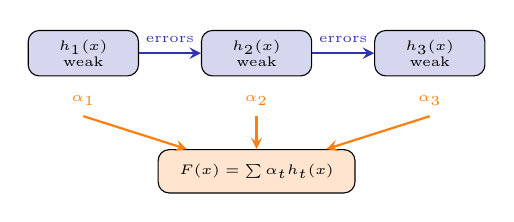
\begin{tikzpicture}[
  every node/.style={font=\tiny},
  wl/.style={draw,rounded corners,fill=mllavender4,minimum width=1.4cm,minimum height=0.55cm,align=center},
  arr/.style={->,>=stealth,thick,mlpurple}
]
\node[wl] (h1) at (0,0) {$h_1(x)$\\weak};
\node[wl] (h2) at (2.2,0) {$h_2(x)$\\weak};
\node[wl] (h3) at (4.4,0) {$h_3(x)$\\weak};

\draw[arr] (h1) -- (h2) node[midway,above,font=\tiny] {errors};
\draw[arr] (h2) -- (h3) node[midway,above,font=\tiny] {errors};

% Weights
\node[font=\tiny,mlorange] at (0,-0.6) {$\alpha_1$};
\node[font=\tiny,mlorange] at (2.2,-0.6) {$\alpha_2$};
\node[font=\tiny,mlorange] at (4.4,-0.6) {$\alpha_3$};

% Sum
\node[draw,rounded corners,fill=mlorange!20,minimum width=2.5cm,minimum height=0.55cm,align=center,font=\tiny] (sum) at (2.2,-1.5) {$F(x) = \sum \alpha_t h_t(x)$};

\draw[arr,mlorange] (0,-0.8) -- (sum);
\draw[arr,mlorange] (2.2,-0.8) -- (sum);
\draw[arr,mlorange] (4.4,-0.8) -- (sum);
\end{tikzpicture}

\vspace{0.5em}
\scriptsize Sequential: each learner corrects the combined errors of all predecessors.
\end{column}
\end{columns}

\begin{block}{Insight}
\scriptsize Boosting reduces \emph{bias} (makes weak learners strong); bagging reduces \emph{variance} (stabilizes strong learners).
\end{block}
\bottomnote{Schapire (1990) proved that weak learners can be ``boosted'' to arbitrary accuracy.}
\end{frame}

% Frame 20: What Is AdaBoost's Weight Update Rule?
\begin{frame}{What Is AdaBoost's Weight Update Rule?}
\begin{columns}[T]
\begin{column}{0.55\textwidth}
\small
\textbf{Learner weight} (how much to trust learner $t$):
\[
\alpha_t = \frac{1}{2}\ln\frac{1-\epsilon_t}{\epsilon_t}
\]
where $\epsilon_t$ = weighted error rate of $h_t$.

\vspace{0.3em}
\footnotesize
\textbf{Sample weight update} (Freund \& Schapire notation):
\[
w_i \leftarrow w_i \cdot \exp\!\bigl(-\alpha_t \, y_i \, h_t(x_i)\bigr)
\]
where $y_i \in \{-1, +1\}$ and $h_t(x_i)$ is the weak learner prediction.

\begin{compactlist}
\item When $y_i \neq h_t(x_i)$, the exponent is positive, increasing the weight
\item Correctly classified: weight \highlight{decreased}; misclassified: weight \highlight{increased}
\item Next learner focuses on hard examples
\item Normalize weights to sum to 1
\end{compactlist}
\end{column}
\begin{column}{0.42\textwidth}
\footnotesize
\textbf{Properties of $\alpha_t$:}
\begin{compactlist}
\item $\epsilon_t = 0$ (perfect): $\alpha_t \to \infty$
\item $\epsilon_t = 0.5$ (random): $\alpha_t = 0$ (ignored)
\item $\epsilon_t > 0.5$: $\alpha_t < 0$ (inverted)
\end{compactlist}

\vspace{0.5em}
\textbf{Final prediction:}
\[
H(x) = \text{sign}\!\left(\sum_{t=1}^{T} \alpha_t \, h_t(x)\right)
\]

\vspace{0.3em}
\scriptsize AdaBoost is equivalent to forward stagewise additive modeling with exponential loss.
\end{column}
\end{columns}

\begin{block}{Insight}
\scriptsize AdaBoost's exponential loss makes it sensitive to outliers and label noise -- a key limitation in noisy financial data.
\end{block}
\bottomnote{Freund \& Schapire (1997): ``A Decision-Theoretic Generalization of On-Line Learning.'' JCSS.}
\end{frame}

% Frame 21: How Does Gradient Boosting Minimize an Arbitrary Loss?
\begin{frame}{How Does Gradient Boosting Minimize an Arbitrary Loss?}
\begin{columns}[T]
\begin{column}{0.55\textwidth}
\small
\textbf{Additive update:}
\[
f_m(x) = f_{m-1}(x) + \eta \cdot h_m(x)
\]
where $h_m$ fits the \highlight{negative gradient} of the loss:
\[
r_{im} = -\frac{\partial L(y_i, f(x_i))}{\partial f(x_i)}\bigg|_{f=f_{m-1}}
\]

\vspace{0.3em}
\footnotesize
\textbf{Squared loss:} $r_{im} = y_i - f_{m-1}(x_i)$ (residuals)

\textbf{Log loss:} $r_{im} = y_i - \sigma(f_{m-1}(x_i))$

\vspace{0.2em}
Learning rate $\eta \in (0,1]$ shrinks each tree's contribution for regularization.
\end{column}
\begin{column}{0.42\textwidth}
\footnotesize
\textbf{Algorithm:}
\begin{enumerate}
\setlength{\itemsep}{1pt}
\item Initialize $f_0(x) = \arg\min_\gamma \sum L(y_i, \gamma)$
\item For $m = 1, \ldots, M$:
\begin{compactlist}
\item Compute pseudo-residuals $r_{im}$
\item Fit tree $h_m$ to $\{(x_i, r_{im})\}$
\item Update: $f_m = f_{m-1} + \eta \cdot h_m$
\end{compactlist}
\item Output $f_M(x)$
\end{enumerate}

\vspace{0.5em}
\textbf{Key hyperparameters:}
\begin{compactlist}
\item $M$: number of boosting rounds
\item $\eta$: learning rate (0.01--0.3)
\item Tree depth: usually 3--8
\end{compactlist}
\end{column}
\end{columns}

\begin{block}{Insight}
\scriptsize Gradient boosting performs \emph{gradient descent in function space} -- each tree is a step toward the loss minimum.
\end{block}
\bottomnote{Friedman (2001): ``Greedy Function Approximation: A Gradient Boosting Machine.'' Annals of Statistics.}
\end{frame}

% Frame 22: What Makes XGBoost's Objective Function Special?
\begin{frame}{What Makes XGBoost's Objective Function Special?}
\begin{columns}[T]
\begin{column}{0.55\textwidth}
\small
\textbf{Regularized objective:}
\[
\mathcal{L} = \sum_{i=1}^{n} L(y_i, \hat{y}_i) + \sum_{k=1}^{K} \Omega(f_k)
\]
where the regularization term is:
\[
\Omega(f) = \gamma T + \tfrac{1}{2}\lambda\|w\|^2
\]

\vspace{0.2em}
\footnotesize
\begin{compactlist}
\item $T$ = number of leaves, $w$ = leaf weights
\item $\gamma$ penalizes tree complexity (pruning)
\item $\lambda$ penalizes large leaf values (L2)
\end{compactlist}
\end{column}
\begin{column}{0.42\textwidth}
\footnotesize
\textbf{Second-order Taylor expansion:}
\[
\mathcal{L}^{(t)} \approx \sum_{i} \bigl[g_i f_t(x_i) + \tfrac{1}{2}h_i f_t^2(x_i)\bigr] + \Omega(f_t)
\]

where $g_i = \partial_{\hat{y}} L$, $h_i = \partial^2_{\hat{y}} L$.

\vspace{0.5em}
\textbf{Optimal leaf weight:}
\[
w_j^* = -\frac{\sum_{i \in I_j} g_i}{\sum_{i \in I_j} h_i + \lambda}
\]

\vspace{0.3em}
\scriptsize Using second-order info gives faster convergence than first-order gradient boosting.
\end{column}
\end{columns}

\begin{block}{Insight}
\scriptsize XGBoost's regularization prevents overfitting \emph{structurally} (fewer leaves) and \emph{numerically} (smaller weights) -- crucial for noisy financial data.
\end{block}
\bottomnote{Chen \& Guestrin (2016): ``XGBoost: A Scalable Tree Boosting System.'' KDD.}
\end{frame}

%% === SECTION 6: EVALUATION ===

% Frame 23: When Does a Forest Fail Silently?
\begin{frame}{When Does a Forest Fail Silently?}
\begin{columns}[T]
\begin{column}{0.55\textwidth}
\small
Four failure modes that produce \highlight{no error message} but wrong predictions:

\vspace{0.3em}
\footnotesize
\begin{compactlist}
\item \textbf{Extrapolation:} RF cannot predict outside training range (piecewise constant). New market regimes break the model.
\item \textbf{Class imbalance:} 99.9\% legitimate $\Rightarrow$ ``always predict legit'' achieves 99.9\% accuracy but catches zero fraud.
\item \textbf{Feature leakage:} Future information in training features (e.g., post-transaction flags) inflates apparent accuracy.
\item \textbf{Concept drift:} Fraud patterns evolve; a model trained in 2023 degrades by 2024.
\end{compactlist}
\end{column}
\begin{column}{0.42\textwidth}
\scriptsize
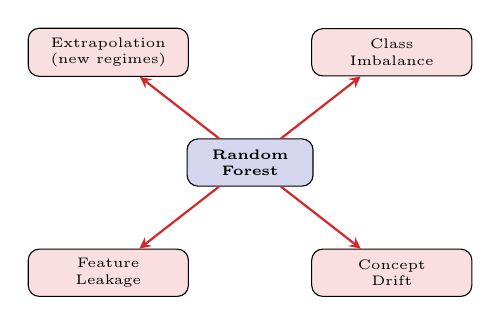
\begin{tikzpicture}[
  every node/.style={font=\tiny},
  risk/.style={draw,rounded corners,fill=mlred!15,text width=1.8cm,align=center,minimum height=0.6cm},
  center/.style={draw,rounded corners,fill=mllavender4,minimum width=1.6cm,minimum height=0.6cm,align=center,font=\tiny\bfseries}
]
\node[center] (rf) at (0,0) {Random\\Forest};
\node[risk] (ex) at (-1.8,1.4) {Extrapolation\\(new regimes)};
\node[risk] (ci) at (1.8,1.4) {Class\\Imbalance};
\node[risk] (fl) at (-1.8,-1.4) {Feature\\Leakage};
\node[risk] (cd) at (1.8,-1.4) {Concept\\Drift};

\draw[->,>=stealth,thick,mlred] (rf) -- (ex);
\draw[->,>=stealth,thick,mlred] (rf) -- (ci);
\draw[->,>=stealth,thick,mlred] (rf) -- (fl);
\draw[->,>=stealth,thick,mlred] (rf) -- (cd);
\end{tikzpicture}

\vspace{0.5em}
\scriptsize All four produce high accuracy on historical data but fail in production.
\end{column}
\end{columns}

\begin{block}{Insight}
\scriptsize Always evaluate on \emph{temporally out-of-sample} data and monitor model performance continuously in production.
\end{block}
\bottomnote{Silent failures are worse than crashes -- they erode trust slowly and cause regulatory risk.}
\end{frame}

% Frame 24: How Do You Choose the Right Hyperparameters?
\begin{frame}{How Do You Choose the Right Hyperparameters?}
\begin{columns}[T]
\begin{column}{0.55\textwidth}
\small
\renewcommand{\arraystretch}{1.15}
\footnotesize
\begin{tabular}{@{}lll@{}}
\toprule
\textbf{Param} & \textbf{Default} & \textbf{Guideline} \\
\midrule
n\_estimators & 100 & 500+; more is rarely worse \\
max\_depth & None & Limit to 10--20 for speed \\
min\_samples\_split & 2 & Increase to reduce overfit \\
max\_features & $\sqrt{p}$ & Try $\log_2 p$ for large $p$ \\
class\_weight & None & `balanced' for imbalance \\
\bottomrule
\end{tabular}

\vspace{0.5em}
\begin{compactlist}
\item \textbf{Tuning order:} max\_features $\to$ max\_depth $\to$ n\_estimators
\item Use OOB score for quick evaluation
\item Use cross-validation for final selection
\end{compactlist}
\end{column}
\begin{column}{0.42\textwidth}
\footnotesize
\textbf{Overfitting signals:}
\begin{compactlist}
\item Training accuracy $\gg$ test accuracy
\item OOB error diverges from training error
\item Feature importance dominated by noise features
\end{compactlist}

\vspace{0.5em}
\textbf{Underfitting signals:}
\begin{compactlist}
\item Both training and test accuracy low
\item Increase max\_depth or n\_estimators
\item Check if max\_features is too small
\end{compactlist}

\vspace{0.5em}
\scriptsize
\textbf{Rule of thumb:} Start with defaults, increase n\_estimators to 500, then tune max\_features via grid search.
\end{column}
\end{columns}

\begin{block}{Insight}
\scriptsize Random Forests are remarkably robust to hyperparameters -- defaults often perform within 1--2\% of the optimum.
\end{block}
\bottomnote{Probst et al.\ (2019): ``Hyperparameters and Tuning Strategies for Random Forest.'' WIREs Data Mining.}
\end{frame}

%% === SECTION 7: FINANCE APPLICATION ===

% Frame 25: How Do Fraud Teams Use Feature Importance for Transaction Monitoring?
\begin{frame}{How Do Fraud Teams Use Feature Importance for Transaction Monitoring?}
\begin{columns}[T]
\begin{column}{0.55\textwidth}
\small
\textbf{Worked case study:}

\vspace{0.2em}
\footnotesize
\textbf{Features:} transaction amount, merchant category, time of day, customer age, distance from home, transaction frequency (last 24h), card-present flag.

\vspace{0.3em}
\textbf{Model:} RF with 500 trees, class\_weight=`balanced', trained on 6 months of labeled data.

\vspace{0.3em}
\textbf{Top-5 by permutation importance:}
\begin{enumerate}
\setlength{\itemsep}{1pt}
\item Distance from home ($\Delta$AUC = 0.08)
\item Transaction amount ($\Delta$AUC = 0.06)
\item Frequency last 24h ($\Delta$AUC = 0.04)
\item Time of day ($\Delta$AUC = 0.03)
\item Card-present flag ($\Delta$AUC = 0.02)
\end{enumerate}
\end{column}
\begin{column}{0.42\textwidth}
\footnotesize
\textbf{Actionable insights:}
\begin{compactlist}
\item \textbf{Distance:} Transactions far from home are the strongest fraud signal
\item \textbf{Amount:} Large transactions need extra scrutiny, but amount alone is insufficient
\item \textbf{Frequency:} Rapid-fire transactions suggest card testing
\item \textbf{Time:} Late-night transactions correlate with fraud
\item \textbf{Card-present:} CNP (card-not-present) transactions are riskier
\end{compactlist}

\vspace{0.5em}
\scriptsize These findings are presented to fraud analysts as SHAP waterfall plots for each flagged transaction.
\end{column}
\end{columns}

\begin{block}{Insight}
\scriptsize Feature importance tells analysts \emph{where to look}; SHAP tells them \emph{why this specific transaction} was flagged.
\end{block}
\bottomnote{Fraud teams combine model outputs with rule-based systems for final decisions.}
\end{frame}

% Frame 26: What Happens When 99.9% of Transactions Are Legitimate?
\begin{frame}{What Happens When 99.9\% of Transactions Are Legitimate?}
\begin{columns}[T]
\begin{column}{0.55\textwidth}
\small
\textbf{The class imbalance problem:}
\begin{compactlist}
\item Fraud rate $\approx$ 0.1\% $\Rightarrow$ 1 fraud per 1000 transactions
\item Classifier predicting ``always legit'' gets 99.9\% accuracy
\item \highlight{Accuracy is meaningless} for imbalanced data
\end{compactlist}

\vspace{0.3em}
\footnotesize
\textbf{Solutions:}
\begin{compactlist}
\item \texttt{class\_weight='balanced'}: upweight minority class inversely proportional to frequency
\item \textbf{Stratified bootstrap:} ensure each tree's sample has proportional fraud cases
\item \textbf{SMOTE:} synthetic minority oversampling (creates new fraud examples by interpolation)
\item \textbf{Cost-sensitive learning:} $C_{\text{FN}} \gg C_{\text{FP}}$ (missing fraud costs more than false alarms)
\end{compactlist}
\end{column}
\begin{column}{0.42\textwidth}
\footnotesize
\textbf{Precision-recall tradeoff:}
\begin{compactlist}
\item \textbf{Precision:} Of flagged transactions, how many are actually fraud?
\item \textbf{Recall:} Of all fraud, how many did we catch?
\item Lowering threshold $\Rightarrow$ higher recall, lower precision
\item Banks target \highlight{high recall} (catch fraud) at acceptable precision
\end{compactlist}

\vspace{0.5em}
\textbf{Key metrics for imbalanced data:}
\begin{compactlist}
\item PR-AUC (precision-recall curve area)
\item F1 or $F_\beta$ score (weighted harmonic mean)
\item Cost-weighted accuracy
\end{compactlist}
\end{column}
\end{columns}

\begin{block}{Insight}
\scriptsize In fraud detection, a false negative (missed fraud) costs 10--100x more than a false positive (unnecessary alert).
\end{block}
\bottomnote{Use PR-AUC, not ROC-AUC, when the positive class is rare (Davis \& Goadrich, 2006).}
\end{frame}

% Frame 27: When Should You Choose RF Over Logistic Regression?
\begin{frame}{When Should You Choose RF Over Logistic Regression?}
\begin{columns}[T]
\begin{column}{0.55\textwidth}
\small
\textbf{What you see:} A decision flowchart guiding model selection based on data characteristics and requirements.

\vspace{0.3em}
\footnotesize
\textbf{Key pattern:}
\begin{compactlist}
\item \textbf{Interpretability required?} $\Rightarrow$ Logistic regression or single tree
\item \textbf{Nonlinear relationships?} $\Rightarrow$ RF or boosting
\item \textbf{Many features, few samples?} $\Rightarrow$ RF (implicit feature selection)
\item \textbf{Maximum accuracy needed?} $\Rightarrow$ XGBoost with tuning
\end{compactlist}

\vspace{0.3em}
\textbf{Takeaway:} No single model dominates; the right choice depends on the problem, data, and regulatory constraints.
\end{column}
\begin{column}{0.42\textwidth}
\includegraphics[width=\textwidth]{07_decision_flowchart/chart.pdf}
\end{column}
\end{columns}

\begin{block}{Insight}
\scriptsize In regulated industries, the ``best'' model is often the one that is \emph{explainable enough} to satisfy compliance -- not the most accurate.
\end{block}
\bottomnote{Many banks use RF internally but report logistic regression coefficients to regulators.}
\end{frame}

%% === SECTION 8: STAKEHOLDERS ===

% Frame 28: Who Wins and Who Loses When Ensembles Replace Scorecards?
\begin{frame}{Who Wins and Who Loses When Ensembles Replace Scorecards?}
\begin{columns}[T]
\begin{column}{0.55\textwidth}
\small
\begin{compactlist}
\item \textbf{Fraud Team:} Wins -- better detection rates, fewer missed cases, faster adaptation
\item \textbf{Risk Manager:} Wins -- lower losses, better capital allocation, richer risk models
\item \textbf{Compliance:} Mixed -- improved outcomes but harder to audit 500-tree models
\item \textbf{Customer:} Mostly wins -- fewer false declines, but less transparent decisions
\item \textbf{Regulator:} Concerned -- demands explainability, adverse action reasons, fairness audits
\end{compactlist}
\end{column}
\begin{column}{0.42\textwidth}
\scriptsize
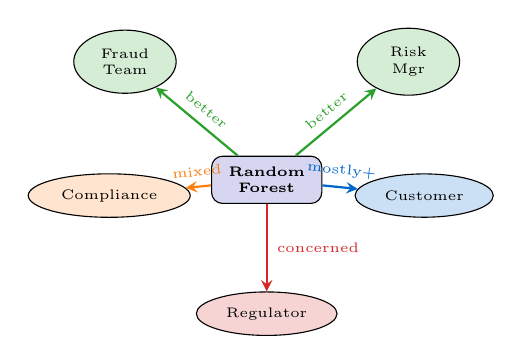
\begin{tikzpicture}[
  every node/.style={font=\tiny},
  center/.style={draw,rounded corners,fill=mlpurple!20,minimum width=1.4cm,minimum height=0.6cm,align=center,font=\tiny\bfseries},
  actor/.style={draw,ellipse,minimum width=1.3cm,minimum height=0.55cm,align=center}
]
\node[center] (rf) at (0,0) {Random\\Forest};
\node[actor,fill=mlgreen!20] (ft) at (-1.8,1.5) {Fraud\\Team};
\node[actor,fill=mlgreen!20] (rm) at (1.8,1.5) {Risk\\Mgr};
\node[actor,fill=mlorange!20] (co) at (-2.0,-0.2) {Compliance};
\node[actor,fill=mlblue!20] (cu) at (2.0,-0.2) {Customer};
\node[actor,fill=mlred!20] (re) at (0,-1.7) {Regulator};

\draw[->,>=stealth,thick,mlgreen] (rf) -- (ft) node[midway,above,sloped,font=\tiny] {better};
\draw[->,>=stealth,thick,mlgreen] (rf) -- (rm) node[midway,above,sloped,font=\tiny] {better};
\draw[->,>=stealth,thick,mlorange] (rf) -- (co) node[midway,above,sloped,font=\tiny] {mixed};
\draw[->,>=stealth,thick,mlblue] (rf) -- (cu) node[midway,above,sloped,font=\tiny] {mostly+};
\draw[->,>=stealth,thick,mlred] (rf) -- (re) node[midway,right,font=\tiny] {concerned};
\end{tikzpicture}
\end{column}
\end{columns}

\begin{block}{Insight}
\scriptsize The transition from scorecards to ensembles is a \emph{governance} challenge as much as a technical one.
\end{block}
\bottomnote{Successful adoption requires buy-in from all five stakeholders, not just data scientists.}
\end{frame}

% Frame 29: Can Regulators Trust a Model Made of 500 Trees?
\begin{frame}{Can Regulators Trust a Model Made of 500 Trees?}
\begin{columns}[T]
\begin{column}{0.55\textwidth}
\small
\textbf{Regulatory landscape:}
\begin{compactlist}
\item \textbf{ECOA / Reg B (US):} Lenders must provide specific ``adverse action reasons'' for denial -- hard with a forest
\item \textbf{GDPR Article 22 (EU):} Right to ``meaningful information about the logic involved'' in automated decisions
\item \textbf{EU AI Act:} High-risk AI systems (credit scoring) require transparency and human oversight
\end{compactlist}

\vspace{0.3em}
\footnotesize
\textbf{Bridging the gap with SHAP:}
\begin{compactlist}
\item SHAP provides per-decision explanations
\item Top-$k$ SHAP features $\Rightarrow$ adverse action reasons
\item Global SHAP summary $\Rightarrow$ model documentation
\end{compactlist}
\end{column}
\begin{column}{0.42\textwidth}
\footnotesize
\textbf{Practical compliance workflow:}
\begin{enumerate}
\setlength{\itemsep}{2pt}
\item Train RF for optimal performance
\item Compute SHAP values for every prediction
\item Map top SHAP features to human-readable reason codes
\item Document model in a ``model risk management'' framework
\item Monitor for fairness across protected classes
\end{enumerate}

\vspace{0.5em}
\scriptsize SR 11-7 (Fed) requires banks to validate and document all models used in decision-making.
\end{column}
\end{columns}

\begin{block}{Insight}
\scriptsize SHAP turns a ``black box'' into a ``glass box'' -- the model is complex, but each decision is explainable.
\end{block}
\bottomnote{The EU AI Act (2024) classifies credit scoring as ``high-risk'' -- requiring explainability by law.}
\end{frame}

%% === SECTION 9: SUMMARY ===

% Frame 30: Key Takeaways
\begin{frame}{Key Takeaways}
\begin{columns}[T]
\begin{column}{0.55\textwidth}
\small
\begin{block}{Mathematical Foundation}
\begin{compactlist}
\item Gini impurity and entropy guide tree splits; both yield similar results
\item Variance of ensemble: $\rho\sigma^2 + \frac{(1-\rho)}{B}\sigma^2$ -- decorrelation is key
\item OOB error provides free, unbiased validation
\end{compactlist}
\end{block}

\vspace{0.3em}
\begin{block}{Ensemble Methods Compared}
\begin{compactlist}
\item \textbf{Bagging/RF:} reduces variance via parallel, decorrelated trees
\item \textbf{AdaBoost:} reduces bias via sequential reweighting
\item \textbf{Gradient Boosting:} gradient descent in function space
\item \textbf{XGBoost:} adds regularization and second-order optimization
\end{compactlist}
\end{block}
\end{column}
\begin{column}{0.42\textwidth}
\small
\begin{block}{Practical Application}
\begin{compactlist}
\item Feature importance: MDI $\to$ permutation $\to$ SHAP (increasing reliability)
\item Fraud detection demands high recall, cost-sensitive learning, and PR-AUC evaluation
\item Class imbalance: class\_weight, SMOTE, stratified sampling
\item SHAP bridges the gap between model complexity and regulatory explainability
\end{compactlist}
\end{block}
\end{column}
\end{columns}
\bottomnote{Random Forests remain one of the strongest ``out-of-the-box'' classifiers two decades after Breiman (2001).}
\end{frame}

% Frame 31: Until Next Time...
\begin{frame}{Until Next Time\ldots}
\begin{columns}[T]
\begin{column}{0.55\textwidth}
\small
We opened with the absurdity of ensemble models (XKCD \#1885).

\vspace{0.5em}
Now you know \highlight{WHY} 500 trees beat one: \textbf{variance reduction through decorrelation}.

\vspace{0.5em}
\footnotesize
\begin{compactlist}
\item One tree is interpretable but fragile
\item Bagging stabilizes via bootstrap averaging
\item Feature randomization decorrelates trees ($\rho \downarrow$)
\item Boosting attacks bias where RF attacks variance
\item SHAP makes the forest explainable for regulators
\end{compactlist}

\vspace{0.5em}
\small
\textbf{Next: L05 -- PCA \& t-SNE}\\
\footnotesize From ensemble predictions to \highlight{dimensionality reduction} -- how to visualize and compress high-dimensional financial data.
\end{column}
\begin{column}{0.42\textwidth}
\includegraphics[height=0.45\textheight]{images/1885_ensemble_model.png}

\vspace{0.5em}
\scriptsize
\textit{``The real power of ensemble models is not that each tree is good -- it is that each tree is wrong in a different way.''}
\end{column}
\end{columns}
\bottomnote{L05 preview: PCA finds directions of maximum variance; t-SNE preserves local structure for visualization.}
\end{frame}

\end{document}
